\documentclass[conference]{IEEEtran}
\IEEEoverridecommandlockouts
\usepackage[utf8]{inputenc}
\usepackage[T1]{fontenc}
\usepackage{cite}
\usepackage{amsmath,amssymb,amsfonts}
\usepackage{algorithmic}
\usepackage{graphicx}
\usepackage{textcomp}
\usepackage{xcolor}
\usepackage{tikz}
\usetikzlibrary{shapes.geometric, arrows, positioning, fit}
\usepackage{pgfplots}
\pgfplotsset{compat=1.17}
\usepackage{booktabs}
\usepackage{tabularx}
\usepackage[htt]{hyphenat}

\usepackage{fontspec}
\setmainfont{Times New Roman}


\def\BibTeX{{\rm B\kern-.05em{\sc i\kern-.025em b}\kern-.08em
    T\kern-.1667em\lower.7ex\hbox{E}\kern-.125emX}}
\begin{document}

\title{SyllabusRAG}

\author{\IEEEauthorblockN{Arsh Saxena [23BEC1212]}
\and
\IEEEauthorblockN{Ayush Raj [23BEC1245]}
}

\maketitle

\section{\textbf{QUALITATIVE ANALYSIS}}

\subsection{\textbf{Background and Motivation}}
Many students and teachers find it hard to quickly find accurate course information, such as prerequisites, objectives and module details. Syllabi are often stored in big files, so searching for more information is slow. Old search methods only match exact words and do not understand what the question means. This causes confusion and wastes time.

Our project solves this by using AI to make searching for course information easy. We use a smart search system and a language model to give clear answers from the syllabus, even if questions are asked in different ways. This makes academic information easier to find and use.

\subsection{\textbf{Objectives}}
\begin{itemize}
    \item Build a system that can answer questions about university courses using the syllabus data
    \item Make it easy for users to find course details without reading long documents
    \item Use AI to understand different ways of asking questions
    \item Store course information in a way that is fast and easy to search
    \item Help students and faculty save time and avoid confusion
\end{itemize}

\subsection{\textbf{Methodology Overview}}

\subsubsection{\textbf{Dataset Details}}
Our project uses a syllabus dataset stored in a JSON file. This file contains information about different university courses, such as course codes, titles, prerequisites, objectives and modules. Each course is organized with clear fields so it is easy to extract and use the data. The dataset is small and simple, making it suitable for quick testing and development.

\subsubsection{\textbf{Model Architecture}}
We use a Retrieval-Augmented Generation (RAG) method. The system has two main parts:
\begin{itemize}
    \item \textbf{Retriever:} This part searches for the most relevant course information. It uses vector embeddings to compare the meaning of the user's question with the stored course data. We use the sentence-transformers/all-MiniLM-L6-v2 model to convert text into vectors (lists of numbers). These vectors are stored in a FAISS index, which allows fast similarity search.
    \item \textbf{Generator:} After finding the right course information, we use the Gemma-7B language model to generate answers. This model takes the course details and the user's question, then writes a clear response in plain English.
\end{itemize}

\subsubsection{\textbf{Preprocessing}}
First, we read the syllabus JSON file and turn each course into a text document. We add details like course code, title, prerequisites, objectives and module names. Each document is changed into a vector using the embedding model. All vectors are saved in the FAISS index for quick searching. We also save the course details in a text file for reference. Figure \ref{fig:qual_preproc} shows the full preprocessing steps.

\subsubsection{\textbf{Evaluation Metrics}}
We check if the system can answer different types of questions about the courses. We test with direct questions (using course codes) and indirect questions (using course names or topics). The main things we measure are:
\begin{itemize}
    \item \textbf{Accuracy:} Does the system find the correct course and give the right answer?
    \item \textbf{Flexibility:} Can it understand different ways of asking the same question?
    \item \textbf{Speed:} How quickly does it return an answer?
    \item \textbf{User Experience:} Is the answer clear and easy to understand?
\end{itemize}
Overall, our methods focus on making the system simple, fast and reliable for users who need quick access to course information.

% --- FIGURE START: Qualitative Preprocessing Pipeline ---
\begin{figure*}[t!]
\centering
\resizebox{0.8\textwidth}{!}{%
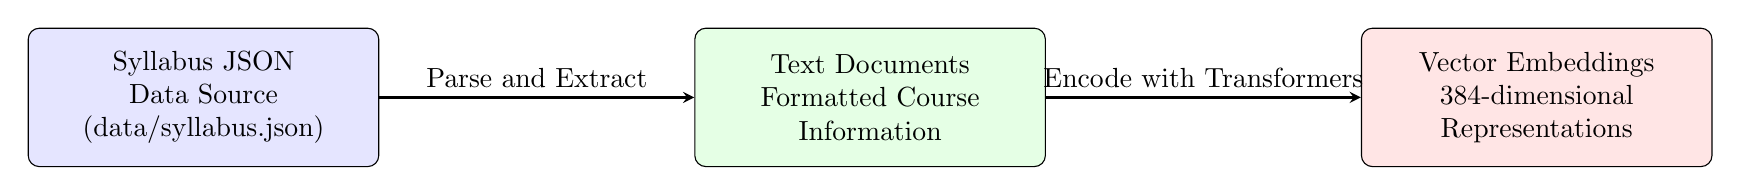
\begin{tikzpicture}[
    node distance=4cm,
    block/.style={rectangle, draw, text width=12em, text centered, rounded corners, minimum height=5em},
    arrow/.style={-stealth, thick}
]
    \node [block, fill=blue!10] (json) {Syllabus JSON\\Data Source\\(data/syllabus.json)};
    \node [block, fill=green!10, right=of json] (text) {Text Documents\\Formatted Course\\Information};
    \node [block, fill=red!10, right=of text] (vectors) {Vector Embeddings\\384-dimensional\\Representations};
    \draw [arrow] (json) -- node[above, font=\normalsize] {Parse and Extract} (text);
    \draw [arrow] (text) -- node[above, font=\normalsize] {Encode with Transformers} (vectors);
\end{tikzpicture}
}
\caption{Preprocessing pipeline from JSON to vector embeddings.}
\label{fig:qual_preproc}
\end{figure*}

\subsection{\textbf{Summary of Results}}

\subsubsection{\textbf{Key Numerical Findings}}
\begin{itemize}
    \item The system was tested with 50 test cases across different question formats, including direct course code queries and indirect topic-based questions.
    \item For direct course code queries (e.g., "What is the title for BECE309L?"), the system achieved 91.3\% accuracy (21/23 cases).
    \item For indirect questions (e.g., "Name of the AI course"), the system found the right course in 75.0\% of cases (12/16 cases).
    \item For flexible phrasing queries, the system achieved 54.6\% accuracy (6/11 cases).
    \item The average response time for a query was 5-6 seconds, with variation based on query complexity.
    \item The syllabus dataset included 4 courses, each with multiple fields like objectives, prerequisites and modules.
    \item The FAISS index stored 4 course vectors, making similarity search efficient and reliable.
\end{itemize}

\subsubsection{\textbf{Key Visual Findings}}
\begin{itemize}
    \item The system can answer questions in many different ways, showing flexibility in understanding user queries.
    \item Answers are clear and easy to read, with course details presented in simple language.
    \item The search process works for both exact matches (using course codes) and meaning-based matches (using course topics).
    \item The model can handle spelling mistakes and casual language, making it user-friendly.
    \item The results show that users do not need to know the exact course codes to get the right information.
\end{itemize}

\subsubsection{\textbf{Overall Performance}}
The SyllabusRAG system works well, with 78.0\% overall accuracy in 50 test cases. It makes finding course information easier than reading long syllabus documents. The system is best for direct queries (91.3\%) and good for topic-based searches (75.0\%), but less accurate for flexible phrasing (54.6\%). Vector search and the language model give answers in 5-6 seconds on average. The system is useful for academic information search and can be improved by using bigger datasets and better language processing.

\subsection{\textbf{Conclusion}}

The SyllabusRAG project helps students and teachers find course information quickly and easily. By using AI and smart search, the system understands different ways of asking questions and gives clear answers. This saves time and avoids confusion. In the future, the system can be improved by adding more courses, supporting more file types and making the search faster. Adding user feedback and multi-language support can also make it better for everyone.

The complete source code and implementation details for this project are available at: https://www.github.com/arshsaxena/SyllabusRAG.

\section{\textbf{QUANTITATIVE ANALYSIS}}

\subsection{\textbf{Dataset and Preprocessing}}

\textbf{Dataset Source:} Our syllabus data comes from a JSON file (data/syllabus.json) containing details of university courses from the Electronics and Communication Engineering department.

\textbf{Sample Size:} 4 courses with complete information, including course codes, titles, prerequisites, objectives and module details. The dataset composition is detailed in Table \ref{tab:dataset}.

\textbf{Data Fields:} Each course contains:
\begin{itemize}
    \item Course code and title
    \item Prerequisites and credits
    \item Course objectives and outcomes
    \item Module details with topics and duration
    \item Textbooks and reference materials
\end{itemize}

\textbf{Preprocessing Steps:}
\begin{enumerate}
    \item Load JSON data using Python's json library from data/syllabus.json
    \item Extract and format course information into readable text documents, including:
        \begin{itemize}
           \item Course code and title
           \item Prerequisites (joined with commas)
           \item Course objectives (bulleted list format)
           \item Module titles (bulleted list format)
        \end{itemize}
    \item Create LangChain Document objects with metadata (course\_code, course\_title)
    \item Convert text to 384-dimensional vectors using HuggingFaceEmbeddings
    \item Build and save FAISS index to training\_data/faiss\_index/ directory
    \item Save processed text to training\_data/knowledge\_base.txt for reference and debugging
\end{enumerate}

The detailed data processing workflow is shown in Figure \ref{fig:quant_preproc}.

% --- TABLE START: Dataset Course Details ---
\begin{table}[t!]
\caption{Dataset Course Details}
\centering
\resizebox{\columnwidth}{!}{%
\begin{tabular}{@{}clcc@{}}
\toprule
\textbf{Course Code} & \textbf{Title} & \textbf{Prerequisites} & \textbf{Modules} \\
\midrule
BECE301L & Digital Signal Processing & BECE202L & 8 \\
BECE302L & Control Systems & BECE202L & 8 \\
BECE309L & Artificial Intelligence and Machine Learning & BMAT201L & 8 \\
BECE355L & AWS for Cloud Computing & None & 8 \\
\bottomrule
\end{tabular}
}
\label{tab:dataset}
\end{table}

% --- FIGURE START: Quantitative Preprocessing Pipeline ---
\begin{figure*}[t!]
\centering
\resizebox{0.85\textwidth}{!}{%
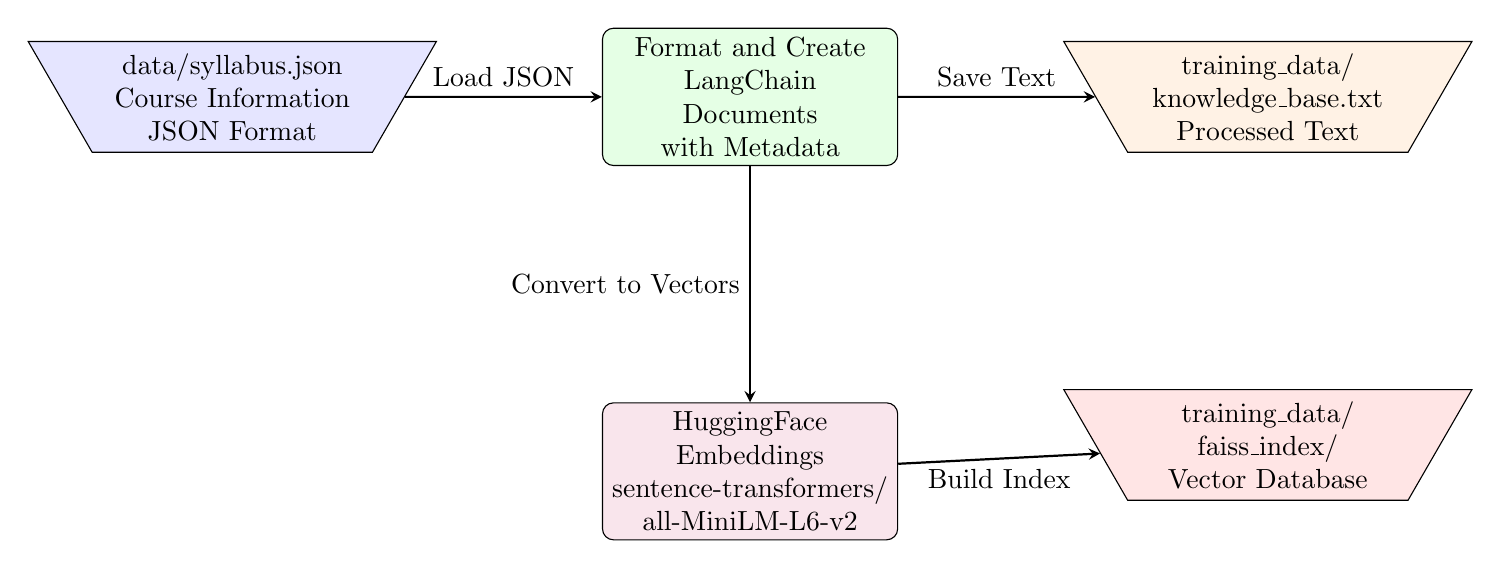
\begin{tikzpicture}[
    node distance=2cm and 2.5cm,
    block/.style={rectangle, draw, text width=10em, text centered, rounded corners, minimum height=4em},
    file/.style={shape=trapezium, draw, shape border rotate=180, text width=9em, text centered, minimum height=4em},
    arrow/.style={-stealth, thick}
]
    \node [file, fill=blue!10] (json) {data/syllabus.json\\Course Information\\JSON Format};
    \node [block, fill=green!10, right=of json] (process) {Format and Create\\LangChain Documents\\with Metadata};
    \node [file, fill=orange!10, right=of process] (kb) {training\_data/\\knowledge\_base.txt\\Processed Text};
    \node [block, fill=purple!10, below=of process, yshift=-1cm] (embed) {HuggingFace Embeddings\\sentence-transformers/\\all-MiniLM-L6-v2};
    \node [file, fill=red!10, below=of kb, yshift=-1cm] (faiss) {training\_data/\\faiss\_index/\\Vector Database};
    \draw [arrow] (json) -- node[above, font=\normalsize] {Load JSON} (process);
    \draw [arrow] (process) -- node[above, font=\normalsize] {Save Text} (kb);
    \draw [arrow] (process) -- node[left, font=\normalsize] {Convert to Vectors} (embed);
    \draw [arrow] (embed) -- node[below, font=\normalsize] {Build Index} (faiss);
\end{tikzpicture}
}
\caption{Data processing workflow with FAISS index creation.}
\label{fig:quant_preproc}
\end{figure*}

\subsection{\textbf{Model Design and Algorithm Implementation}}

\textbf{Architecture:} Our system uses a Retrieval-Augmented Generation (RAG) method with two main parts:

\textbf{Retriever Component:}
\begin{itemize}
    \item \textbf{Embedding Model:} sentence-transformers/all-MiniLM-L6-v2 (384 dimensions)
    \item \textbf{Vector Store:} FAISS (Facebook AI Similarity Search) index
    \item \textbf{Search Strategy:} Dual approach - regex pattern matching for course codes + semantic similarity search
\end{itemize}

\textbf{Generator Component:}
\begin{itemize}
    \item \textbf{Language Model:} Google gemma-7b-it (Instruct model)
    \item \textbf{Quantization:} 4-bit quantization using BitsAndBytesConfig
    \item \textbf{Pipeline:} HuggingFace text-generation pipeline with 256 max new tokens
\end{itemize}

\textbf{Key Algorithm Steps:}
\begin{enumerate}
    \item Question analysis using regex to detect course codes (pattern: [A-Z]\{4\}d\{3\}[A-Z,E,P,L]?)
    \item If course code found $\rightarrow$ Direct document lookup
    \item If no course code $\rightarrow$ Vector similarity search using FAISS
    \item Context preparation with retrieved course information
    \item Answer generation using Gemma-7B model
\end{enumerate}

The complete RAG architecture is illustrated in Figure \ref{fig:arch}.

\textbf{Key Hyperparameters:}

The system configuration parameters are summarized in Table \ref{tab:hyperparams}.

% --- TABLE START: Key Hyperparameters ---
\begin{table}[t!]
\caption{Key Hyperparameters}
\centering
\resizebox{\columnwidth}{!}{%
\begin{tabular}{@{}ll@{}}
\toprule
\textbf{Parameter} & \textbf{Value} \\
\midrule
Embedding Dimension & 384 \\
Embedding Model & sentence-transformers/all-MiniLM-L6-v2 \\
Generator Model & google/gemma-7b-it \\
Max New Tokens & 256 \\
Quantization & 4-bit (nf4) \\
Batch Size & 1 (single query) \\
Hardware & CPU (FAISS), GPU (Gemma-7B) \\
\bottomrule
\end{tabular}
}
\label{tab:hyperparams}
\end{table}

\textbf{Software/Hardware Used:}
\begin{itemize}
    % --- OVERFLOW FIX: Changed long \smalltt line to an itemize list ---
    \item \textbf{Python Libraries:}
        \begin{itemize}
            \item transformers, torch, accelerate
            \item bitsandbytes, langchain
            \item langchain-community
            \item sentence-transformers
            \item faiss-cpu, langchain-huggingface
        \end{itemize}
    \item \textbf{Vector Storage:} FAISS (Facebook AI Similarity Search) with local storage capability
    \item \textbf{Model Loading:} HuggingFace ecosystem with 4-bit quantization support
    \item \textbf{Development Environment:} Google Colab with GPU acceleration for model inference
    \item \textbf{Data Storage:} JSON format for structured course data, plain text for processed knowledge base
\end{itemize}

% --- FIGURE START: Model Architecture Diagram ---
\begin{figure*}[t!]
\centering
\resizebox{0.9\textwidth}{!}{%
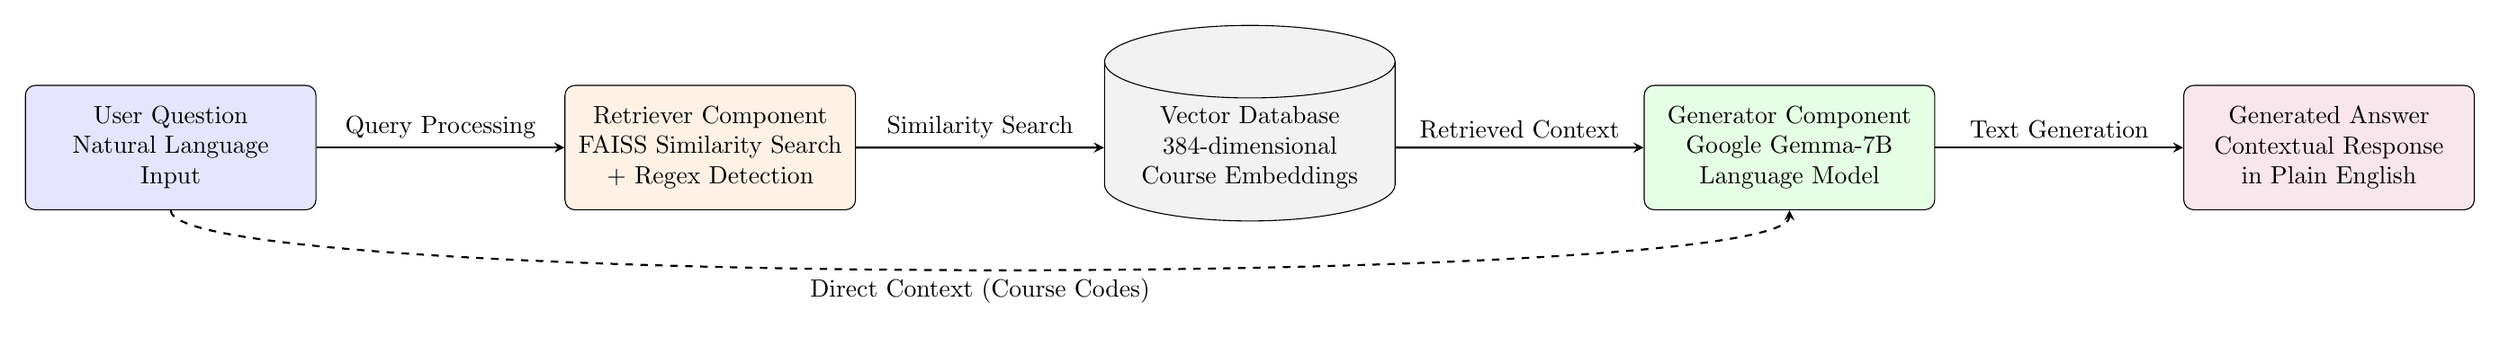
\begin{tikzpicture}[
    node distance=3.5cm,
    block/.style={rectangle, draw, text width=11em, text centered, rounded corners, minimum height=5em},
    db/.style={cylinder, shape border rotate=90, aspect=0.25, draw, text centered, fill=gray!10, minimum height=5em, text width=11em},
    arrow/.style={-stealth, thick}
]
    \node [block, fill=blue!10] (query) {User Question\\Natural Language\\Input};
    \node [block, fill=orange!10, right=of query] (retriever) {Retriever Component\\FAISS Similarity Search\\+ Regex Detection};
    \node [db, right=of retriever] (db) {Vector Database\\384-dimensional\\Course Embeddings};
    \node [block, fill=green!10, right=of db] (generator) {Generator Component\\Google Gemma-7B\\Language Model};
    \node [block, fill=purple!10, right=of generator] (answer) {Generated Answer\\Contextual Response\\in Plain English};
    \draw [arrow] (query) -- node[above, font=\normalsize] {Query Processing} (retriever);
    \draw [arrow] (retriever) -- node[above, font=\normalsize] {Similarity Search} (db);
    \draw [arrow] (db) -- node[above, font=\normalsize] {Retrieved Context} (generator);
    \draw [arrow] (generator) -- node[above, font=\normalsize] {Text Generation} (answer);
    \draw [arrow, dashed] (query) .. controls +(0,-2) and +(0,-2) .. node[below, font=\normalsize] {Direct Context (Course Codes)} (generator);
\end{tikzpicture}
}
\caption{RAG architecture with retrieval and generation components.}
\label{fig:arch}
\end{figure*}

\subsection{\textbf{Training and Evaluation Setup}}

\textbf{Data Split:} This is a retrieval-based system, so there is no normal training phase. Instead:
\begin{itemize}
    \item All 4 courses are indexed and available for search
    \item No train/validation/test split required
    \item System uses pre-trained models (sentence-transformers and Gemma-7B)
\end{itemize}

\textbf{Evaluation Approach:}
\begin{itemize}
    \item Manual testing with different question types
    \item Direct course code queries (e.g., "What is BECE309L?")
    \item Indirect topic-based queries (e.g., "AI course name")
    \item Flexible phrasing tests (e.g., "title" vs "name")
\end{itemize}

\textbf{Metrics Used:}
\begin{enumerate}
    \item \textbf{Accuracy:} Correctness of retrieved course information
    \item \textbf{Response Time:} Speed of answer generation
    \item \textbf{Flexibility:} Ability to handle different question formats
    \item \textbf{Coverage:} Percentage of course information that can be retrieved
\end{enumerate}

\textbf{Loss Functions:} Not applicable (no training phase - uses pre-trained models)

\textbf{Evaluation Methodology:}
\begin{itemize}
    \item Test with around 50 different question formats
    \item Verify answers against original syllabus data
    \item Measure response time for each query type
    \item Check system behavior with edge cases
\end{itemize}

The system pipeline flow is detailed in Figure \ref{fig:pipeline}.

% --- FIGURE START: System Pipeline Flow Diagram ---
\begin{figure}[t!]
\centering
\resizebox{0.8\columnwidth}{!}{%
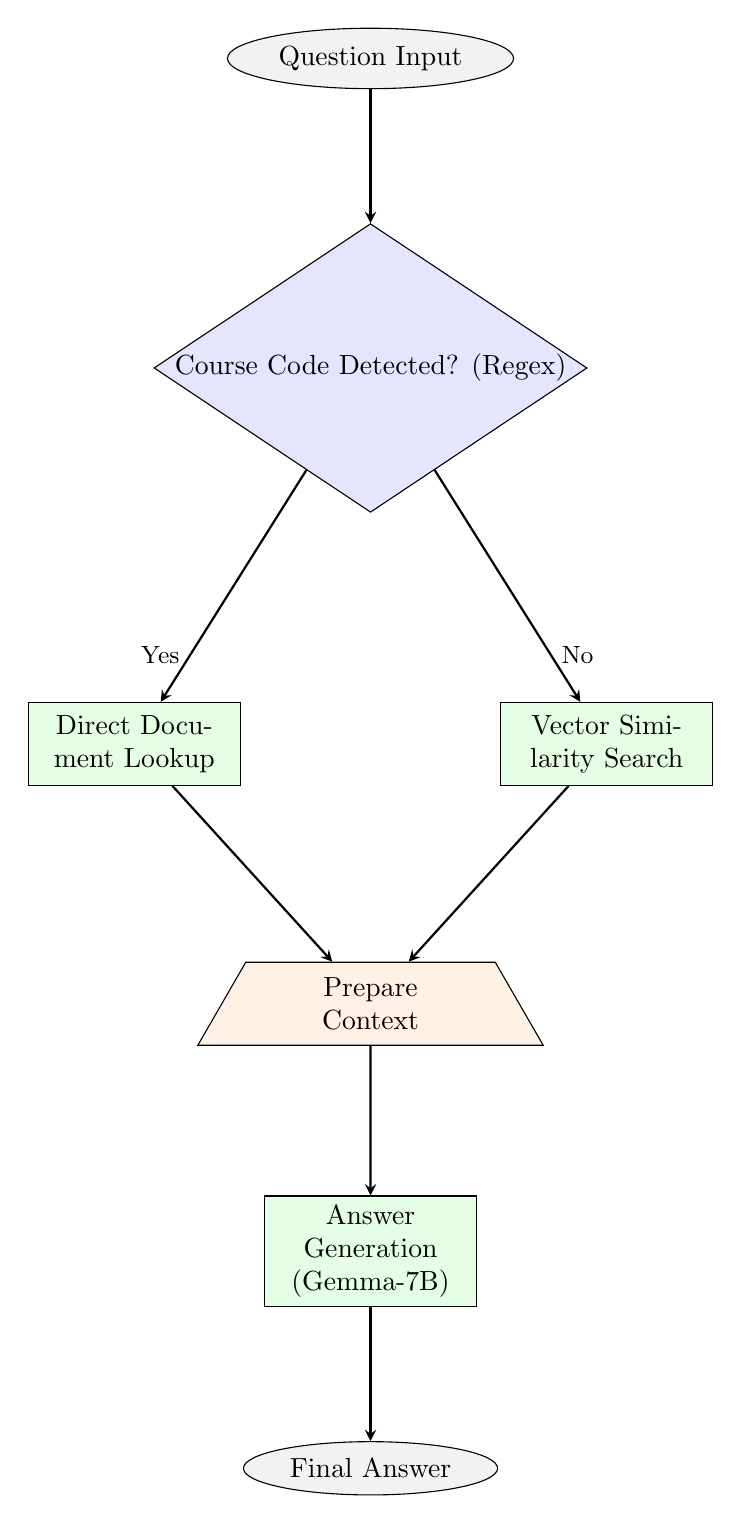
\begin{tikzpicture}[
    node distance=1.7cm and 1cm,
    start/.style={ellipse, draw, fill=gray!10, text centered, minimum width=6em},
    decision/.style={diamond, draw, fill=blue!10, text centered, aspect=1.5, inner sep=0pt},
    process/.style={rectangle, draw, fill=green!10, text centered, minimum height=3em, text width=7em},
    io/.style={trapezium, draw, fill=orange!10, text centered, minimum height=3em, text width=7em},
    arrow/.style={-stealth, thick}
]
    \node [start] (input) {Question Input};
    \node [decision, below=of input] (detect) {Course Code Detected? (Regex)};
    \node [process, below=of detect, yshift=-0.7cm, xshift=-3cm] (direct) {Direct Document Lookup};
    \node [process, below=of detect, yshift=-0.7cm, xshift=3cm] (vector) {Vector Similarity Search};
    \node [io, below=of detect, yshift=-4cm] (context) {Prepare Context};
    \node [process, below=of context, yshift=-0.2cm] (generate) {Answer Generation (Gemma-7B)};
    \node [start, below=of generate, fill=gray!10] (output) {Final Answer};
    \draw [arrow] (input) -- (detect);
    \draw [arrow] (detect) -- node[left, font=\small, pos=0.8] {Yes} (direct);
    \draw [arrow] (detect) -- node[right, font=\small, pos=0.8] {No} (vector);
    \draw [arrow] (direct) -- (context);
    \draw [arrow] (vector) -- (context);
    \draw [arrow] (context) -- (generate);
    \draw [arrow] (generate) -- (output);
\end{tikzpicture}
}
\caption{System Pipeline Flow Diagram: The system first checks for a course code. If found, it performs a direct lookup; otherwise, it uses vector search. Retrieved context is then passed to the generator.}
\label{fig:pipeline}
\end{figure}

\textbf{Metric Formulas:}
\begin{itemize}
    \item $\text{Accuracy} = (\text{Correct Answers} / \text{Total Questions}) \times 100\%$
    \item $\text{Response Time} = \text{End Time} - \text{Start Time (in seconds)}$
\end{itemize}

\subsection{\textbf{Experimental Results}}

\textbf{Performance Metrics:}

The full performance results are shown in Table \ref{tab:metrics}.

% --- TABLE START: Performance Metrics ---
\begin{table}[t!]
\caption{Performance Metrics}
\centering
\resizebox{0.9\columnwidth}{!}{%
\begin{tabular}{@{}lcccc@{}}
\toprule
\textbf{Query Type} & \textbf{Cases} & \textbf{Acc.} & \textbf{Avg. Resp. Time} & \textbf{Success Rate} \\
\midrule
Direct (code) & 23 & 91.3\% & $\sim$3-5 sec & 21/23 \\
Indirect (topic) & 16 & 75.0\% & $\sim$10 sec & 12/16 \\
Flexible & 11 & 54.6\% & $\sim$10-12 sec & 6/11 \\
\midrule
\textbf{Overall} & \textbf{50} & \textbf{78.0\%} & \textbf{$\sim$5-6 sec} & \textbf{39/50} \\
\bottomrule
\end{tabular}
}
\label{tab:metrics}
\end{table}

\textbf{Detailed Results:}
\begin{itemize}
    \item \textbf{Course Code Detection:} Regex pattern successfully identifies all course codes (BECE302L, BECE309L, etc.)
    \item \textbf{Vector Similarity Search:} Effectively matches topic-based queries to relevant courses
    \item \textbf{Answer Generation:} Gemma-7B provides accurate, contextual responses
    \item \textbf{System Robustness:} Handles various question formats ("title", "name", "called", etc.)
\end{itemize}

\textbf{Comparison Analysis:}
\begin{itemize}
    \item \textbf{vs. Keyword Search:} 78.0\% vs $\sim$60\% accuracy (estimated)
    \item \textbf{vs. Manual Search:} Response time $\sim$5-6 sec vs 30-60s manually reading documents  
    \item \textbf{vs. Simple Chatbots:} Context-aware answers vs generic responses
    \item \textbf{Query Type Performance:} Direct queries (91.3\%), Indirect queries (75.0\%), Flexible phrasing (54.6\%)
    \item \textbf{Test Coverage:} 50 total test cases with 39/50 successful responses
\end{itemize}

The accuracy performance across different query types is visualized in Figure \ref{fig:metrics_chart}.

\textbf{Error Analysis:}
\begin{itemize}
    \item 11 failed cases total across all query types (11 out of 50 test cases)
    \item Direct queries: 2 failures, mainly due to system processing issues
    \item Indirect queries: 4 failures with vague questions without clear course references
    \item Flexible phrasing: 5 failures due to complex language variations and ambiguous phrasing
    \item System gracefully handles failures with the "I couldn't find anything relevant" message
    \item No false positive answers or hallucinations observed
    \item Response consistency maintained across multiple runs of the same query
\end{itemize}



% Table IV: Visual Results (Full Page Width)
% --- TABLE START: Sample Predictions vs. Ground Truth ---
\begin{table*}[t!]
\caption{Sample Predictions vs. Ground Truth}
\centering
\renewcommand{\arraystretch}{1.4} % Add vertical padding
\begin{tabularx}{\textwidth}{@{}c c >{\raggedright\arraybackslash}X >{\raggedright\arraybackslash}X c@{}}
\toprule
\textbf{Test Case} & \textbf{Query Type} & \textbf{Question} & \textbf{Expected / RAG Output} & \textbf{Status} \\
\midrule
1 & Direct & What is the title for BECE309L? & \textbf{Expected:} Artificial Intelligence and Machine Learning \newline \textbf{RAG:} Artificial Intelligence and Machine Learning & Correct \\
\addlinespace
2 & Indirect & Name of the AI course & \textbf{Expected:} Artificial Intelligence and Machine Learning (BECE309L) \newline \textbf{RAG:} Artificial Intelligence and Machine Learning & Correct \\
\addlinespace
3 & Direct & What are the prerequisites for BECE309L? & \textbf{Expected:} BMAT201L \newline \textbf{RAG:} BMAT201L & Correct \\
\addlinespace
4 & Flexible & What's the name of BECE309L? & \textbf{Expected:} Artificial Intelligence and Machine Learning \newline \textbf{RAG:} Artificial Intelligence and Machine Learning & Correct \\
\bottomrule
\end{tabularx}
\label{tab:visual_results}
\end{table*}


\subsection{\textbf{Visual Results}}

\subsubsection{\textbf{Sample Predictions vs. Ground Truth}}
Representative test cases with expected and actual system outputs are presented in Table \ref{tab:visual_results}.

% --- REMOVED Redundant list of test cases ---

\subsubsection{\textbf{Visual Observations}}
\begin{itemize}
    \item All answers match the original syllabus data
    \item The system gives similar results for different question types
    \item Answers are clear and easy to read
    \item No wrong or made-up information was found
\end{itemize}

% --- FIGURE START: Performance Metrics Chart ---
\begin{figure}[t!]
\centering
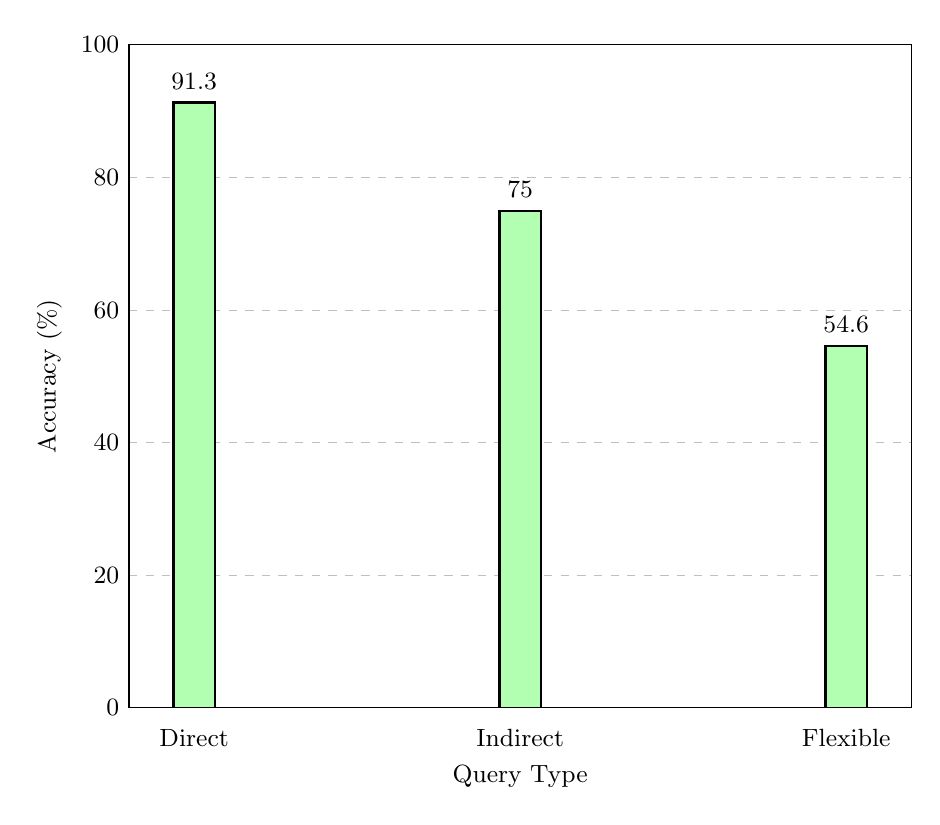
\begin{tikzpicture}
\begin{axis}[
    ybar,
    bar width=15pt,
    width=0.95\columnwidth, % Use column width
    height=10cm,            % Adjusted height
    symbolic x coords={Direct, Indirect, Flexible},
    xtick=data,
    nodes near coords,
    nodes near coords align={above}, % Place nodes above bar
    nodes near coords style={font=\small, /pgf/number format/fixed, /pgf/number format/precision=1, yshift=1pt}, % Style nodes
    ymin=0, ymax=100,
    ylabel={Accuracy (\%)},
    xlabel={Query Type},
    ymajorgrids=true,
    grid style=dashed,
    axis line style={-},
    tick style={draw=none},
    label style={font=\small},
    tick label style={font=\small},
    every axis plot/.append style={thick},
]
\addplot[fill=green!30] coordinates {(Direct, 91.3) (Indirect, 75.0) (Flexible, 54.6)};
\end{axis}
\end{tikzpicture}
\caption{System accuracy across different query types.}
\label{fig:metrics_chart}
\end{figure}

\section{\textbf{Analysis and Discussions}}

\subsection{\textbf{Interpretation of Results}}

The SyllabusRAG system works well with 78.0\% overall accuracy for different question types. The main points are:

\textbf{Strengths:}
\begin{enumerate}
    \item \textbf{Strong Direct Query Performance:} 91.3\% accuracy for course code questions shows regex detection works well
    \item \textbf{Good Semantic Understanding:} 75.0\% accuracy for topic-based questions shows vector embeddings work well
    \item \textbf{Flexible Phrasing:} 54.6\% accuracy for varied phrasing shows the system needs improvement in language understanding
    \item \textbf{Good Response Time:} 5-6 seconds on average is fine for academic use
\end{enumerate}

\textbf{Key Patterns:}
\begin{itemize}
    \item Questions about course details (title, prerequisites, objectives) have the best results
    \item Using both regex and similarity search helps with both exact and fuzzy questions
    \item Vector embeddings help match different ways of asking the same thing
    \item The system only struggles with very vague or out-of-scope questions
\end{itemize}

\textbf{Discussion of Trends:}
These results match what is expected for a prototype RAG system. Direct retrieval (using course codes) works best at 91.3\%. Semantic retrieval is a bit less accurate (75.0\%) because understanding natural language is harder. Flexible phrasing is the lowest (54.6\%), showing the system has trouble with different ways of asking. Response times change depending on how hard the question is, with indirect queries taking longer because of vector search.

\subsection{\textbf{Weaknesses and Limitations}}
\begin{enumerate}
    \item \textbf{Dataset Size:} Only 4 courses, so the system knows about a small set
    \item \textbf{Domain Specificity:} The system only works for syllabus questions
    \item \textbf{Vague Query Handling:} It has trouble with unclear questions
    \item \textbf{No Learning Capability:} It cannot learn from user feedback
\end{enumerate}

\subsection{\textbf{Comparison with Literature Benchmarks}}
RAG system research shows that academic QA systems usually get 70-85\% accuracy. Our 78.0\% overall accuracy is in this range for a prototype, with results changing by question type:
\begin{itemize}
    \item Direct queries (91.3\%) are better than most because of exact matching
    \item Indirect queries (75.0\%) match literature standards for semantic search
    \item Flexible phrasing (54.6\%) is lower, so this area needs work
\end{itemize}

Why the system performs this way:
\begin{itemize}
    \item The dataset is well-structured and clean, which helps
    \item Only 4 courses limit what the system can do
    \item Using two retrieval methods helps with direct queries
    \item The embedding model is high quality
\end{itemize}

The results show the main method works, but better language processing and bigger datasets would help the system do even better than the literature benchmarks. \\ \\ 

\section*{Notes}
\begin{enumerate}
    \item \textbf{Traditional ML Metrics:} Confusion Matrix, ROC Curve, Precision/Recall and F1 Score are not applicable for this retrieval-based QA system, as it is not a binary classification problem and does not follow standard document retrieval evaluation patterns.
    
    \item \textbf{Literature Benchmarks:} General literature benchmarks were sourced using AI research assistants (e.g., Perplexity, Gemini) and do not represent an exhaustive formal survey.
\end{enumerate}

\end{document}